\subsection{Cart}

%For the main pages put a mockup and describe it in detail.

%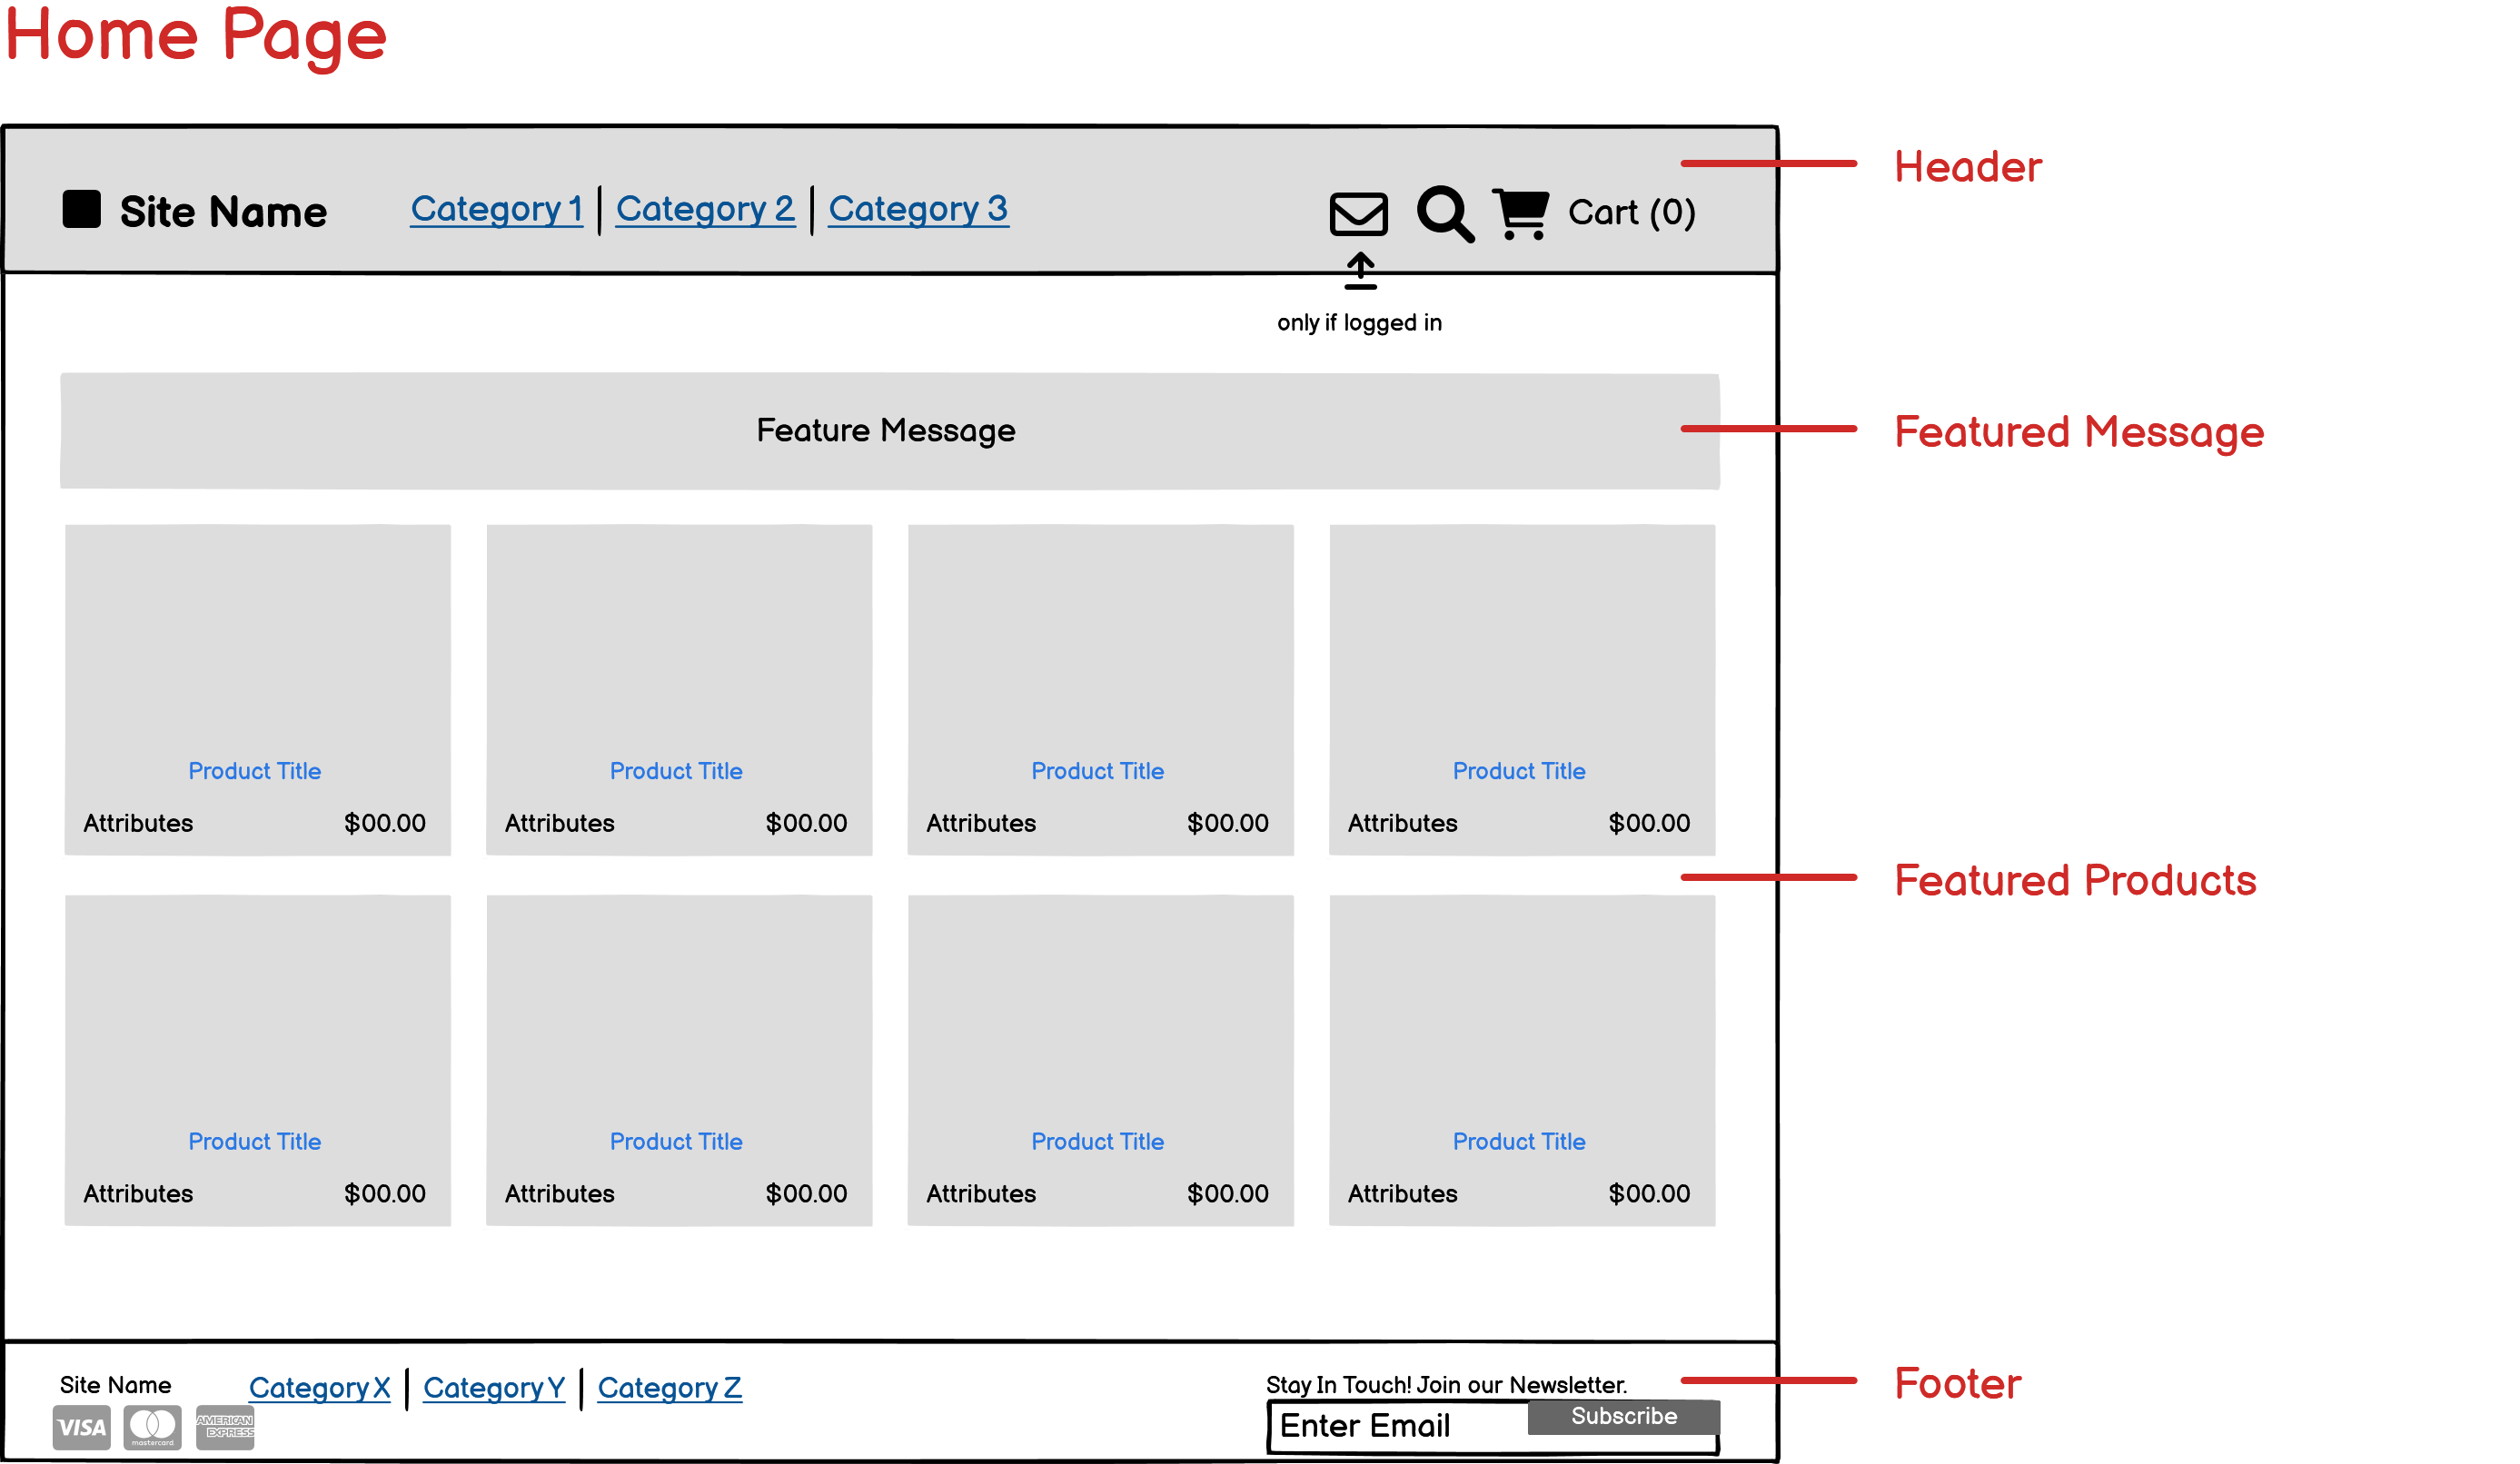
\includegraphics[scale=0.5]{logos/Images/pages/Home Page.png}

\begin{figure}[h]
    \centering
    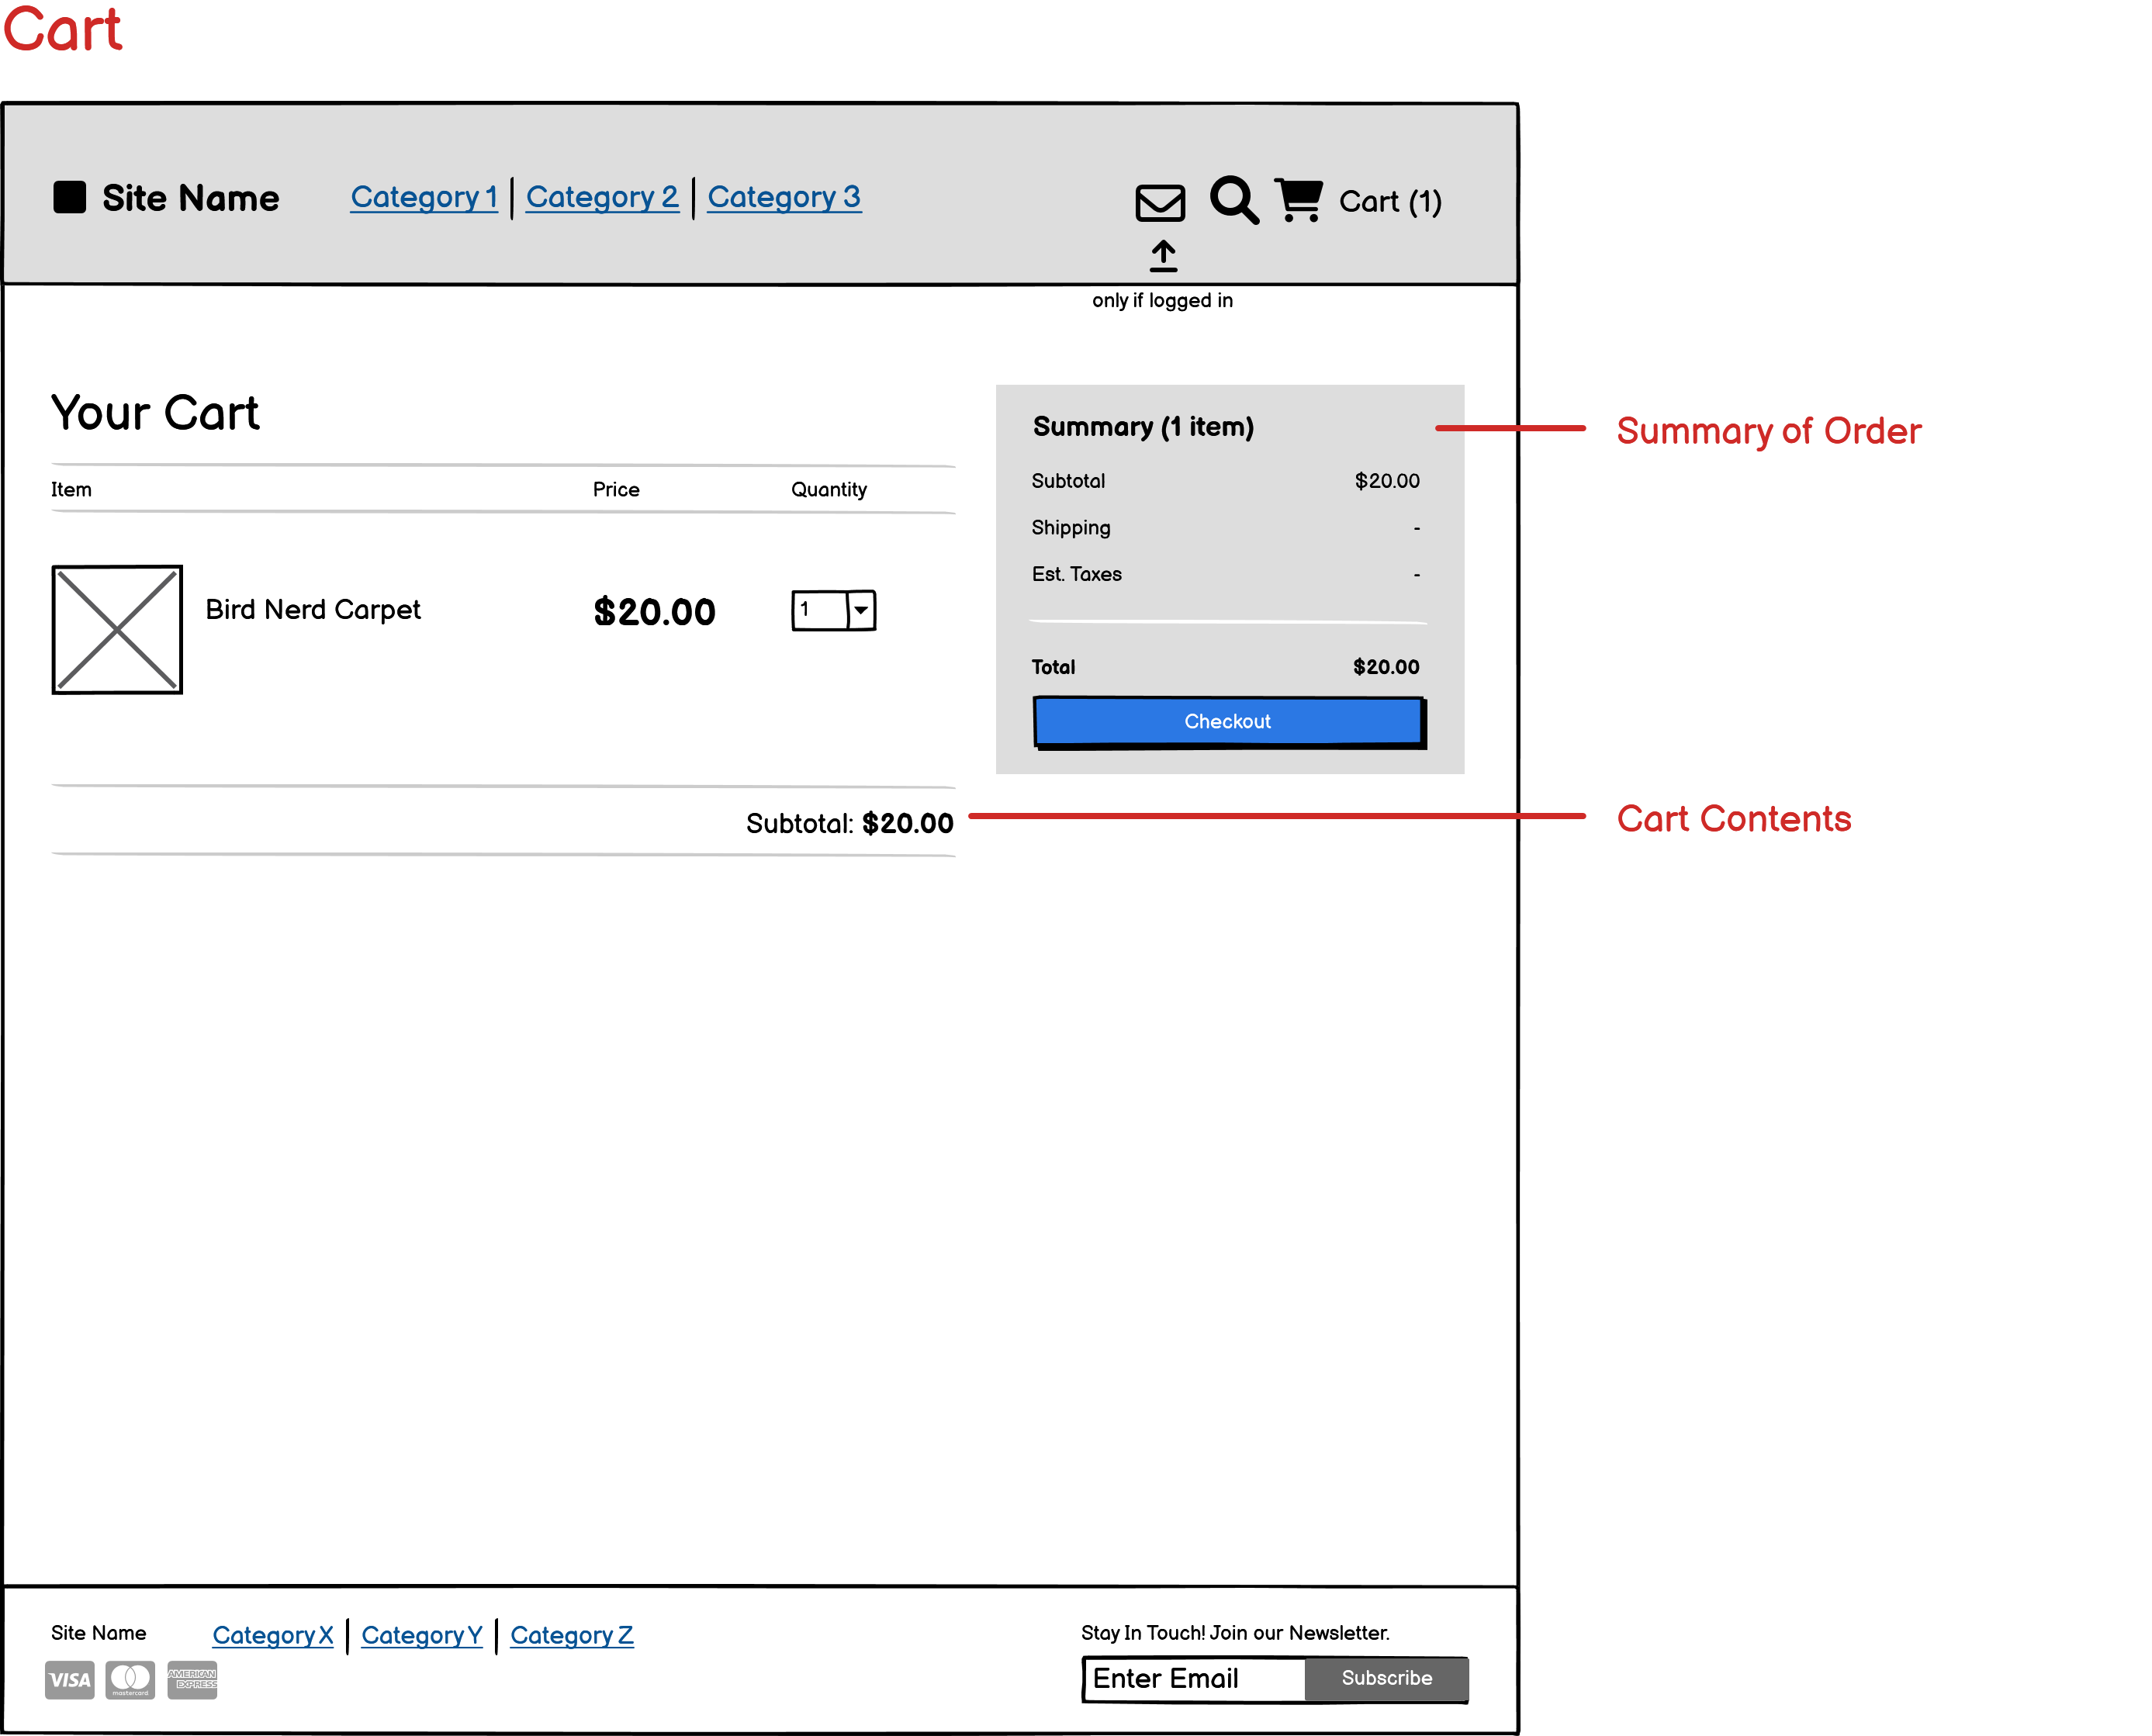
\includegraphics[scale=0.5]{logos/Images/pages/Cart.png}
    \caption{Cart}
    \label{fig:my_label}
\end{figure}
\hfill \break
On the website there is a shopping cart where the selected products are displayed before the order is placed. On the left side, the customer gets an overview of the products that are in the shopping cart, with the respective price and the number of selected items. Furthermore, it is displayed how high the total costs are. The customer can still make changes here, for example, remove items or adjust the quantity. If everything is correct, the customer can click on the "Checkout" button to complete the ordering process and buy the products.